\chapter{Background}
\label{bg}

In this chapter we look at the ways one can represent input data (section \ref{data_rep}), and which models might be used for different input modalities (section \ref{models_considered}). We consider ways to increase label efficiency with active learning (section \ref{bg_al}), and general approaches to effective machine learning (section \ref{bg_general}) as well as combining different models either through joint training or ensembling (section \ref{bg_ensembling}).
Label efficiency can also be achieved through unsupervised or semi-supervised learning, which is described in appendix \ref{unsup_appendix} but is not used in our experiments.

\section{Input Representations}
\label{data_rep}

\subsection{Categorical Input}

The simplest option for representing categorical input is 1-hot encoding, where input has as many dimensions as there are distinct categorical values (vocabulary size); a single dimension is set to 1, with all other dimensions set to 0.
This is a straightforward representation: for a simple model such as logistic regression, we can clearly interpret the model parameters and see how the presence or absence of a given category increases or decreases the likelihood of a given output.
However, in cases where vocabulary sizes get  large, and the number of outputs (the number of units in the next layer in a deep network,  or the number of output units  in a shallow one) increases, this kind of encoding can really blow up the number of parameters of the model.

An alternative is to use  random embeddings:  dense, low-dimensional representations of a high-dimensional vectors.
It has been shown in compressed sensing literature that if a high-dimensional signal in effect lies on a low-dimensional manifold, then the original signal can be reconstructed from a small number of linear measurements \cite{compressive_sensing2}.
This has a useful implication for machine learning: categorical variables with large vocabularies of size \textit{d}  can be  represented with  random embedding vectors of size $M = \log(d)$.
This is because it is possible to reconstruct any d-dimensional k-sparse signal using at most $k  log{\frac{d}{k}}$ dimensional vectors \cite{compressive_sensing1}, and 1-hot vectors are 1-sparse, as only one dimension is nonzero.

An intuitive example is given in \cite{compressive_sensing3} about natural images: a 1-million-pixel image could have roughly 20,000 edges\footnote{Technically: wavelet coefficients with a significant power, which roughly corresponds to a superimposition of edges.}, i.e. it lies in a roughly 20,000-dimensional manifold from which the original image can be constructed with high fidelity.
The 1-million-dimensional image could be projected into a M-dimensional space ``by taking M measurements of the image, where each measurement consists of a weighted sum of all the pixel intensities, and allowing the weights themselves to be chosen randomly (for example, drawn independently from a Gaussian distribution)''\cite{compressive_sensing3}.
The projection is random because the weights for the sum of pixel intensities are chosen randomly.
Why the projections need to be random is motivated by another intuitive example.
When light is shined on a 3-dimensional wireframe, its shadow is a 2-dimensional projection of it.
The projection could lose some important information about the regional object if the direction of the light source is chosen poorly,  however random directions are likely to result in projections where every link of the wire will have a corresponding nonzero length of shadow.

\subsection{Text Input}

The simplest way to represent  text is bag words (\textbf{BoW}),  which  is simply the histogram of word occurrences  in the text.
BoW  representations give equal weight to each of the words in the text, and the model has to learn the relative importance of each of these.
A commonly used representation in information retrieval (IR) is \textbf{TF-IDF},  which stands for ``term frequency -  inverse document frequency''.
TF-IDF  multiplies the term frequency (number of times the word occurred in the text) with its inverse document frequency (the inverse of how often a occurs in all documents).
This has the effect of giving lower scores for common words, and higher scores for words which appear often in a document but not too frequently in the whole corpus.
Another common representation is bag of n-grams (\textbf{BonG}), which  is a histogram of character n-grams.

The above representations are sparse, like 1-hot encoding of categorical variables.
Text can also be  represented as a sequence of \textbf{word embeddings}.
Word embeddings can either be random vectors or representations  learned with word co-occurrence algorithms such as word2vec \cite{word2vec} and GloVe \cite{glove};  these representations can remain fixed throughout the learning procedure, or updated as part of the stochastic gradient descent (SGD) when applicable.
A simple way to represent text is to average the word embedding contained in it.
The  average could also be weighted by the TF-IDF score of each word\footnote{The author is unaware whether this has been tried before, but it seems a promising approach.}.
In \cite{doc2vec}, paragraph vectors are created in a similar manner to word2vec vectors by relying on these vectors to predict the next word in a sentence.

More complex methods use recurrent neural networks (\textbf{RNNs}) to combine a sequence of word embeddings  into a fixed length vector (see section \ref{rnn}).
These kinds of models are good at  disambiguating the potentially many meanings a word might have.
Exactly what gets persisted in the final  vector representation of text depends on how the model is trained - two RNNs  trained on different tasks (such as sentiment analysis and named entity recognition)  would need to store different information in its hidden state to successfully  perform their relevant tasks,  hence the encoding for the same sentence would be different for either model.
Still, an RNN  that is trained on one task could provide useful features for another.
Encoding text as fixed length vectors using RNNs has been interpreted as compressed sensing \cite{compressed_sensing_rnn}, with such vectors being ``provably at least as powerful on classification tasks, up to small error, as a linear classifier over BonG vectors''.

\subsection{Image Input}

Images can be represented as dense 3-dimensional tensor.
A 28x28 RGB image could be represented as a tensor with shape [28, 28, 3],  with the final dimension corresponding to the green, red, and blue intensity values at a given x/y coordinate.
These intensities  are usually in the range 0 ... 255, but are normalised before input to machine learning model.
Similarly to RNNs  encoding a sequence of words to a vector, 2D convolutional neural networks (2D CNNs)  can be used to extract dense feature vectors from raw images (image embedding),  further discussed in section \ref{image_models}.

\section{Models Considered}
\label{models_considered}

The following sections describes a selection of models that could be used for our classification task.
This is by no means an exhaustive list, nor is it a selection that is expected to have the highest predictive performance individually.
These models might become part of an ensemble or be trained jointly with other models, where diversity matters much more than the performance of any individual model.
Engineering  considerations and time constraints also influence the selection of models.
We did not want to spend time implementing nontrivial models from scratch, or to use many frameworks for training models.
TensorFlow  is a widely used machine learning library with a good selection of open source models, in particular a selection of pre-trained models for computer vision and NLP, and has arguably the most mature deployment ecosystem.
Therefore models that did not have an open source TensorFlow implementation or a trivial implementation were excluded.

Section \ref{general_models} describes models that can take categorical and text inputs, section \ref{text_models} looks at some neural models that take only text inputs, and section \ref{image_models} describes 2D CNNs that can classify or extract features from images.

\subsection{General Models}
\label{general_models}



\subsubsection{Logistic Regression}

Logistic regression is a linear, discriminative classifier that is a common baseline model, since it is both interpretable and efficient to train.
There are methods that take time linear in the number of non-zeros in the dataset, which is the smallest amount possible, and it can be made to handle non-linear decision boundaries by using kernels \cite{murphy}.

We have two cases: for independent categorical outputs we use a separate binomial logistic regression model for each output class, and for mutually exclusive classes we use multinomial logistic regression.
This is shown formally in eq  \ref{logistic} and \ref{logistic_binom}, where where \textit{X} and \textit{W} correspond to the input and weight matrices, respectively.

We follow the notational trick where the first row of \textit{X} is always 1, and the first row of \textit{W} corresponds to the bias term.
The loss function of this model as well as how it is optimised is described in section \ref{loss}.

\begin{equation}
\label{logistic}
p(y|X,W)=\mathrm{sigmoid}(W^TX) \
\end{equation}

% todo
\begin{equation}
\label{logistic_binom}
p(y|X,W)=\mathrm{softmax}(W^TX) \
\end{equation}

\subsubsection{Feedforward Neural Network}

Feedforward neural networks (also called deep feedforward networks, multi-layer perceptrons) have been described as function approximator, whose goal is to approximate some functions $f^*$.
We expect some familiarity with neural networks from the reader; for an excellent overview of the various use cases and models of deep learning, refer to \cite{dlb}.
In our case, the input is some representation of categorical, text or image input - often an embedding extracted with another model or assigned randomly.
The hidden layers of our network are homogenous: they use the same activation function (ReLu, sigmoid, or tanh) and have the same number of units;  activation functions and the number of units in hidden layers are determined through hyperparameter tuning.
Similarly to logistic regression, we have two cases: sigmoid activation for independent categories and softmax layer for mutually exclusive categories.

\subsubsection{Wide \& Deep}
\label{bg_wide_deep}

Wide and deep model was originally proposed for recommender systems \cite{wide_deep}, but can just as well be used for classification.
In this model a deep network and a linear logistic regression model are trained jointly in the same SGD learning process, rather than trained separately and then ensembled.
The wide component is good at remembering ``feature interactions through a wide set of cross-product feature transformation'' while the deep model provides good generalisation.
In our experiments we did not use cross products of features.

\subsubsection{Loss Function and Optimizers}
\label{loss}

Logistic regression and neural networks are optimised with some variant of gradient descent.
The loss function was the same for multi-label and multi-class training objectives: binary cross-entropy between the training data and the model distribution, with the loss value averaged across all classes.
This is given in eq. \ref{xentropy}, where $\theta$ corresponds to the model parameters such as the weights and biases of the model, $C$ corresponds to the number of classes, and $P(c=1|x, \theta)$ gives the predicted probability that the item belongs to class $c$ given the feature vector $x$.

\begin{align}
  \label{xentropy}
  NLL(\theta) &= \sum\limits_{c=1}^C \sum\limits_{i=1}^N\left[c_i\log P(c=1|x, \theta) + (1-c_i)\log(P(c=0|x, \theta) )\right]
\end{align}

We are minimising the negative log likelihood (NLL) rather than maximising the product of likelihoods.
Multiplying large numbers of probabilities could result in numerical underflow and rounding errors, therefore it is pragmatic to work with sums of log probabilities instead.
The Adam \cite{adam} optimiser works very well with default hyperparameters, and is therefore used for all stochastic gradient descent updates.

Cross-entropy is a standard loss function for multi-class and multi-label classification, however in our cases it may have downsides.
There is at times ambiguity as to which category a product should belong, therefore even hand-assigned labels are somewhat arbitrary.
The similarity between categories is ignored by this loss function: a short coat that is misclassified as an earring has the same loss value as a coat that is classified as a jacket.
Additionally, the rule-based labels are incomplete: the lack of a label does not always mean that the product does not belong to the given category, yet the model gets penalised for cases where such label is missing but the model correctly predicted a semantically similar class.

The Wasserstein distance metric (also called earth mover distance) can be used instead, which gives the cost of the optimal transport plan for moving the mass of one probability distribution to another.
In our case the two distributions are the label distribution of a data point (1-hot / k-hot vector) and the class distribution predicted by the model.
The optimal transport plan is weighted by a $KxK$ distance matrix, where $K$ is the number of classes and the entries in the matrix correspond to how dissimilar the classes are\footnote{Similarity is known \textit{a priori}, e.g. derived from WordNet hierarchy. It would be interesting to explore similarity matrices created using cosine distance of embedding vectors of categories; embeddings could be extracted with an RNN from the description of the category}.
Intuitively, transporting probability mass from the category ``Coats'' to ``Earrings'' should be more expensive than from ``Coats'' to ``Jackets''.
As there could be many acceptable transport plans that preserve the probability mass, an iterative algorithm needs to be used to find an approximately optimal one that also considers the different cost associated with transporting probability from one class to another.
In \cite{wasserstein_loss} the Sinkhorn-Knopp algorithm with an entropic regularisation term is used as a relaxation of the exact but costly linear programming solution.
This is still an expensive operation compared to cross-entropy or mean squared error, but should be manageable in the ~1000-dimensional space of categories, as opposed to 500x500-dimensional image space where it is often also applied.

% TODO describe why we won't use this loss

\subsection{Text Models}
\label{text_models}

\subsubsection{1D Convolutional Neural Networks}

1D CNNs are a simple yet powerful family of neural models that can work on variable-length sequences of data.
These models convolve several ``filters'' on top of the original sequence, which produce variable-length activations; some (usually max) pooling operation ensures the final activation is of a fixed length.
Therefore such models can be used as classifiers as well as feature extractors.
We do not use 1D CNNs in our experiments; refer to appendix \ref{1d_cnn_app} for a more thorough overview.

\subsubsection{Recurrent Neural Networks}
\label{rnn}

Recurrent neural networks (RNNs) are a another family of models capable of processing sequential data.
RNNs take a sequence of inputs (e.g. dense word embeddings), and either output a prediction after each time step, or after processing the whole sequence.
RNNs and its variants maintain a memory vector that represents the input the model has seen so far; the state of the hidden vector after processing all data points is an embedding of the sequence, which can be used for prediction or in downstream models.
We do not use RNNs in our experiments; refer to appendix \ref{rnn_app} for a more thorough overview.

\subsubsection{Deep Averaging Network}

Deep averaging networks are simple architectures where the embeddings of the input tokens (words, in our case) are averaged and fed through a deep network \cite{dan}.
In fact, a deep model with embedding inputs is very similar to a deep averaging networks, the main difference is in the way the model is optimised and regularised.
We use the Universal Sentence Encoder \cite{uni_sent_enc} in our experiments, which is a deep averaging network pre-trained on a large text corpus.

\subsection{Image Models}
\label{image_models}

2D CNNs are important historically - excellent results in computer vision revived interest and funding in deep learning - but also applicable to a wide range of problems.
Computer vision CNNs tend to be complex models with millions of parameters and hundreds of layers.
It is very compute-intensive and time-consuming to search for new architectures, and the analysis of these is beyond the scope of this work.
Our goal is to use a CNN that has a reasonable performance with decent speed.

The general architecture of a 2D CNN is as follows.
Patches of feature extractors are convolved over the x and y axis of the image; these are often small, e.g. 3x3x$c$ patches that span all the $c$ channels of the image ($c=3$ for RGB images), and convolution could be strided.
Former models used larger patch sizes, but stacking several smaller patches could achieve similar receptive fields while allowing for a larger number of non-linearities for the same number of parameters.
One or more layers of convolutions would be followed by a (often max) pooling layer.
Computer vision architectures tend to re-use the same sub-structure repeatedly: either the same kinds of convolutions followed by pooling, or the ``network in a network'' structure popularised by GoogLeNet \cite{googlenet}.
After a number of such repeated structures, there are normally a few fully-connected layers followed by a softmax or sigmoid layer.

Transfer learning is particularly applicable to computer vision.
Successful computer vision models require a notoriously large training datasets, which would be hard to come by for every problem.
Instead, models are often initialised to the values of a model that has been trained on a large dataset such as ImageNet \cite{imagenet}, excluding only the last layer(s) of the model that has learned features that are specific to the original problem.
Representations learned at the lower layers are remarkably  universal and useful for other tasks.
Therefore pre-trained 2D CNNs can be used as feature extractors for various other tasks,  or the models could be fine-tuned to learn representations that are even more useful to the new task.

\subsection{Downstream Models}

\subsubsection{Item Similarity}
\label{bg_sim}

Similarity measures based on tokenised text are easily accessible to e-commerce companies.
The full-text search engine Lucene is at the core of the popular open source NoSQL database ElasticSearch (ES).
ES provides document similarity metrics that are some combination of normalised TF-IDF vectors between all documents and a query, which could be another document.
This gives decent results in many cases, but it does not take advantage of a product image.

Embeddings extracted with a deep network can be viewed as a distributed representation of the original data, which carries semantic meaning \cite{distributed_reps}.
In the contrived examples of distributed representations, each dimension would represent the degree to which a property (e.g. of shape or colour) is present of an object, however the dimensions are not necessarily so nicely disentangled in the representations learned by deep networks\footnote{The author has not seen strong evidence in literature to support either case, but at least in \cite{towards} extra steps had to be taken to \textit{prevent} certain latent variables from encoding properties of the data that were designed to be captured by other latent variables. This implies that by default, each latent variable contains a little bit of information about each aspect of the input, and that the whole pattern of the embedding matters for conveying semantic information}.
Still, semantically similar data points will have similar embedding vectors, which help shallow models make accurate predictions.

Therefore we can compare any two embedding vectors extracted with the same neural network using standard vector space similarity measures, such as cosine similarity (1 - normalised dot product between the vectors).
Such embeddings can be extracted from product images with 2D CNNs pre-trained on another task, 1D CNNs or RNNs on product title and descriptions, or from the joint embeddings described in section \ref{bg_ensembling}.
With large numbers of products, calculating pairwise similarity scores becomes intractable, therefore approximate nearest neighbour methods could be used \cite{nmslib}.

Another interesting method of computing similarity scores between documents utilises the full-text search capability of tools such as Lucene, which would be valuable to firms already using such technologies.
The embedding vectors of products could be tokenised, by converting each dimension of each embedding vector into tokens that represent the feature with some precision \cite{vec_fulltext}.
For example, we could consider two levels of precision and divide the normalised feature into 10 intervals of size 0.1 and 100 intervals of size 0.01; each product would get two tokens per embedding dimension.
It would be a good idea to also have some wider overlapping intervals as well, e.g. 0 ... 0.5.
For example, if the first embedding dimension is 0.46, the inserted tokens would be d1\_0.4 and d1\_0.46.
Full-text search engines would assign higher scores to co-occurrences in the more precise tokens and lower scores to co-occurrences in more coarse token.

\subsubsection{Recommender Systems}
\label{rec}

Several methods have been proposed that use dense embeddings learned by deep models as part of a recommender algorithm.
These are briefly described here to motivate our focus on models that obtain dense embeddings of products.

Models that deal exclusively with deep embeddings \cite{mvdl} require huge amounts of user-product feedback pairs, therefore the more interesting solutions are ones which work together with classical methods such as matrix factorisation (MF).
MF finds - purely from the implicit or explicit feedback users give to items - vectors of latent factors that represent each user's preferences and each item's ``qualities''; the inner product between a user's and item's latent factors gives a score of compatibility between the two.
Deep models can augment the item latent factors by injecting the embeddings learned for another task.
The main difference in these methods is how the deep embeddings are merged into MF, and how the deep embeddings are obtained in the first place.
In \cite{cdl}, stacked denoising autoencoders are used for unsupervised feature learning of item data, while \cite{dl_mf} uses simply visual embeddings extracted from a 2D CNN pre-trained on ImageNet.

\section{Combining Models}
\label{bg_ensembling}

Individual models can be combined to achieve greater accuracy and lower label complexity; the models can either become a part of an enseble (described in section \ref{ens}), or trained jointly as part of the same gradient descent optimisation process (described in section \ref{joint}).
A neural network can be optimised simultaneously for many objectives; additional training objectives can improve the accuracy of other objectives.
Multi-objective learning (described in section \ref{multiobj}) can be seen as a way of combining the models of individual training objectives.

\subsection{Ensembling}
\label{ens}

Some ensembling approaches  are expected to consist of \textbf{weak learners} or models from the same model family.
Bootstrap aggregation (a.k.a bagging)   draws several bootstrap samples  from the training data,  trains a separate model per bootstrap sample,  and averages the predictions of these individual models.  This reduces the variance of predictions without increasing its bias and generally leads to  more accurate predictors \cite{bagging}.
Boosting is another common meta-algorithm that iteratively trains an ensemble of weak models, such that the data points that incurred a higher error on the previous ensemble are weighted more heavily, and each new weak model is added to the ensemble with a weight proportional to the weak learners accuracy.
A common boosting algorithm is AdaBoost \cite{adaboost}.

We are interested in ways of combining models that are separately trained and combined into a single predictor.
Committee methods and stacked generalisation are more appropriate for \textbf{ensembling strong, independently trained models}.
Simple solutions are voting or (weighted) averaging, where the weights can be found with k-fold cross-validation.
A more appealing approach is stacked generalisation, where a meta-learner is trained on the outputs of the individual models.
This meta-learner could be a relatively simple model, such as logistic regression or a decision tree, and the results of the meta-learner can be therefore quite interpretable.
Refer to figure \ref{ens_vs_joint} for a schema of an ensemble of two neural networks.

\subsection{Joint Training}
\label{joint}

% One orthogonal approach to combining models is joint training of model components.
All models described in section \ref{models_considered} are trained using stochastic gradient descent, so in principle it would be possible to learn the parameters of all components (1D CNN, 2D CNN, RNN, DNN, logistic regression) as part of a single optimisation loop.
This would be an engineering challenge due to the different ways these model require their input to be represented and the large size of the combined model.
In our case this would be clearly an overkill, but it would be an interesting research problem to examine whether joint training has advantages over ensembling in cases where we have different views of the data (in terms of considering different input dimensions or processing the inputs differently).
As mentioned in the Wide \& Deep paper \cite{wide_deep}, the wide component of the model has to just handle cases where the deep component falls short, and can therefore be simpler than it would need to be in an ensemble; analogously, jointly training different neural networks would allow each component to be simpler.

One of the motivations for picking mostly deep neural models was their transfer learning capability.
They all produce a dense embedding vector from which separate logistic or multinomial regressions predict the class.
While it is useful to have separate embeddings for images, text and categorical variables, we would also like to have a compound embedding of each product.
A simple concatenation of all individual embeddings could be a useful (albeit a quite high-dimensional) representation to be used in downstream models.
Alternatively, we could use this concatenation as an input to a neural network, whose goal is to (1) reduce its dimensionality by removing redundant information and (2) predict the output classes from this compressed embedding.
The latter case could act as a replacement for the meta-learner, with the difference that it takes the penultimate (as opposed to the final) layer of each individual model as input.
Refer to figure \ref{ens_vs_joint} for a schema of joint training.

\begin{figure}
  \centering
  \hspace*{-0.2\textwidth}
  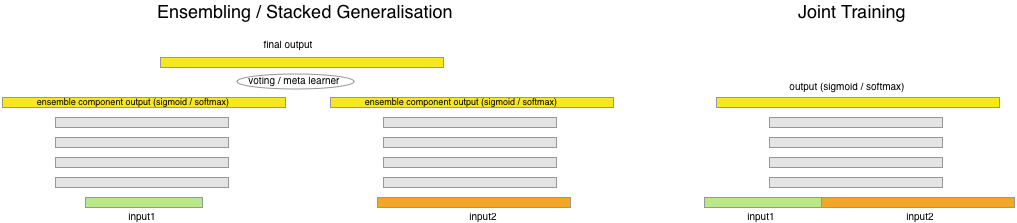
\includegraphics[width=1.4\textwidth]{diagrams/ens_vs_joint}
  \caption{Ensembling / Stacked Generalisation vs Joint Training. Boxes represent inputs (e.g. embedding vectors), hidden layers, and outputs. In ensembles and stacked generalisation (left), we have separate models with no parameter sharing, and the final output is computed either through voting or passing the output of the ensemble components through the meta learner model.  In joint training (right), the two distinct inputs are concatenated and the parameters of the hidden layers are shared.}
  \label{ens_vs_joint}
\end{figure}


\subsection{Multi-Objective Learning}
\label{multiobj}

A neural network can be trained to predict multiple targets from the inputs.
In our setting we can consider the rule-based multi-label objective and the hand-assigned exclusive labels as separate training objectives; we might add additional training objectives that predict colour (multi-label) or conversion (binary).
When using feedforward networks for multi-objective learning, the lower layers are usually shared among the objectives, and the top layers are specific to each training objective.
It has been shown repeatedly that when the training objectives are somewhat related, then adding an additional objective increases the prediction accuracy across the other objectives \cite{multiobj1, multiobj2}.
When implementing multi-objective training, care must be taken not to influence the parameters that are specific to another objective.
Refer to figure \ref{multiobj_model} for a schema of a deep network with two objectives.

\section{Active Learning}
\label{bg_al}

This section describes the main approaches to active learning;  details analysis is beyond the scope of this report.


The goal of active learning is to reduce the number of labels needed  to effectively train a machine learning model by  being selective about which data points to label.
The three general scenarios: membership query synthesis, stream-based selective sampling, and pool-based sampling \cite{al_survey}.
In the first scenario, the algorithm synthesises a datapoint and asks a label for it.
In stream-based selective sampling, and instance is sampled and  the model decides (while having access to the data point's features) whether to acquire a label or not.
In pool-based sampling, the model chooses which data point to label from the pool of all unlabelled samples.
Our use case is a version of pool-based sampling, where the algorithm picks out a batch of products to be labelled.
The rest of the section describes different approaches to picking the data points that are expected to help the model learn.

\textbf{Uncertainty sampling} is the most popular choice: if the model is uncertain about a prediction, obtaining a label for that data point would help it differentiate between different targets.
The most common way to quantify uncertainty is by entropy of the model's predictions:

\begin{equation}
 x^*_H = \argmax_x - \sum_{i} P_\theta(y_i|x) \log P_\theta(y_i|x),
\end{equation}

where $x^*_H$ corresponds to the most informative instance according the entropy ($H$) measure, and $y_i$ corresponds to each class.
% This measure can be used for both multi-label and multi-class problems, and is therefore preferred.

\textbf{Query by committee} uses a number of models trained on the labelled data which all make a prediction on the unlabelled data.
Data points with highest disagreement are expected to be most informative, as by definition a larger number of models would have to be wrong in their predictions.
The models in the committee do not have to be of different type like is our case, but could be e.g. a set of linear classifiers where each committee member just has different parameter values, yet each member would have to be consistent with the current set of labels (not contradict it with its predictions).
Disagreement between committee members can be quantified with vote entropy \cite{vote_entropy}:

\begin{equation}
 x^*_{VE} = \argmax_x - \sum_{i} \frac{V(y_i)}{C}  \log \frac{V(y_i)}{C},
\end{equation}

where $V(y_i)$ is the number of votes given to class $i$ and $C$ is committee size.
Alternatively, KL divergence between each committee member's predictions and the consensus $P_\zeta$ (average prediction of committee members) could be used:

\begin{align}
 x^*_{KL} &= \argmax_x \frac{1}{C} \sum_{i} \infdiv{P_{\theta^{(C)}}}{P_\zeta}\\
 P_\zeta(y_i | x) &= \frac{1}{C} \sum_{c=1}^C P_{\theta^{(C)}}(y_i|x)\\
 \infdiv{P_{\theta^{(C)}}}{P_\zeta} &= \sum_i  P_{\theta^{(C)}}(y_i|x) \log \frac{ P_{\theta^{(C)}}(y_i|x) }{ P_{\zeta}(y_i|x) }
\end{align}

\textbf{Expected model change} calculates how much a model would change if we knew its label.
In gradient-based learning algorithms it is possible to compute the L2 norm of the gradient vector for each combination of labelings of the unlabelled product \cite{model_change}, which is a direct measure of how much the model would change.

\textbf{Expected error reduction} considers how much the test set error is likely to decrease with the acquisition of a given label.
This is done by re-training the model once per each combination of the label values and observing how either the risk or expected log loss of the unlabelled data points decreases.
This is not a suitable use case for deep networks, which are trained over several epochs of the data; there is no efficient way to incrementally train the model, and when re-training with a single additional label, the change in the model is probably higher from the stochasticity in the training procedure rather than the additional label.
In any case, this method is very expensive computationally.

\textbf{Variance reduction} tries to pick data points which are expected to decrease the variance in predictions.
To do that, the Fisher information of the model parameters should be maximised.
Unfortunately this involves inverting a $K \times K$ covariance matrix, where $K$ is the number of parameters in the model.
This is impractical for deep networks with millions of parameters.

\textbf{Information density} measures consider data points that are not just uncertain but also representative of the underlying distribution.
This avoids the problem with many other approaches that ask labels for samples that are controversial, but could otherwise be outliers and not the most useful for good generalisation.
In this framework, a base informativeness measure $\phi_A(x)$ such as uncertainty or disagreement is weighted by the average distance of the data point $x$ to other data points in the distribution:


\begin{equation}
 x^*_{ID} = \argmax_x \phi_A(x) \times \Bigg( \frac{1}{U} \sum_{u=1}^U sim(x, x^{(u)}) \Bigg)^\beta,
\end{equation}

where $sim$ is some similarity function and $\beta$ controls the importance of the density term.

\section{General Practices in Machine Learning}
\label{bg_general}

We briefly list some techniques and approaches that could be used for many kinds of machine learning problems.
Some of these will be used in our experiments, yet some may not be pragmatic due to long train times and time constraints.

Bootstrap sampling, where data points are sampled from training data with replacement, can be used to repeatedly train the same model, and to observe the variance of its predictions.
Bumping can be used to train several models (of the same family) on bootstrap samples to move around in the model space, and will pick the model that best fits the training data.
This helps it explore a wider selection of models, but given that the original training data often also included as one of the bootstrap samples, this method  can still pick the model original model if it happens to have the best accuracy.

There are some versatile methods that can help regularise a neural network, or to speed up convergence by improving  gradient updates.
L2  regularisation should always be used to decrease moral complexity and impose prior on the model parameters, which  implies that very high and very low values are unlikely.
Dropout can mitigate overfitting by preventing neurons from co-adapting, encouraging each to learn representations that are useful independently \cite{dropout}; this has been interpreted as training and exponential (in the number of parameters) number of models and averaging their predictions.
Batch normalisation is known to stabilise training and hence speed up convergence  by normalising each input to have unit variance and zero mean \cite{batch_norm}.
The effect of batch normalisation depends on the minibatch size, so layer normalisation may be used instead ``by computing the mean and variance used for normalization from all of the summed inputs to the neurons in a layer on a single training case'' \cite{layer_norm}.
Gradient clipping has been proposed to alleviate the vanishing and exploding gradient problem notorious in RNNs \cite{grad_clip}.

\subsection{Hyperparameter Tuning Using Bayesian Optimisation}
\label{bayesian_opt}

There are roughly 4 ways of choosing hyperparameters (parameters that are not explicitly learned from the data): manual, grid search, random search and (Bayesian) optimisation.
Some manual choices are done in any case, as one still needs to decide on the intervals for the hyperparameters.
Grid search, where all combinations of (discretised intervals of) hyperparameters is tried, is not scaleable, as the number of possible sets of hyperparameters grows combinatorially; a poor choice of intervals for continuous hyperparameters might miss the ``sweet spot'' for the given parameter, and the model would still need to be evaluated several times for a hyperparameter which has nearly no effect on model performance.
In random search, sets of hyperparameters are sampled uniformly randomly from the given ranges, which is a more efficient use of compute power.
Since each hyperparameter has a distinct value at each train run, this reveals more about how the model's performance changes with respect to all hyperparameters.

The fourth option considers the set of hyperparameters as an input and the model's validation performance as an output to be optimised.
As sampling from this objective function is very expensive - it involves training a neural network until convergence - we need an approach that can explore the space of values efficiently.
We do not have a closed form description of the objective function or gradients of the objective with respect to the inputs, but we can make assumptions about the objective function that can be encoded as priors in a Bayesian framework, e.g. by assuming it has a Gaussian distribution.
To choose sets of hyperparameters that are likely to result in a good performance, the tuning algorithm can use the Bayes rule to compute the posterior distribution of the objective function; points that have a high posterior mean and variance should be explored \cite{bayesian}, as these are the uncertain points that are expected to have the highest value.
